\documentclass[10pt,twocolumn]{article}
	
\usepackage{myfontstyle}
\usepackage{mypackages}
\usepackage{mymacros}
\usepackage{mycommands}
\usepackage{graphicx}
\usepackage{hyperref}
\usepackage{listings}
\usepackage{xcolor}


%%% This defines a style for code blocks (listings package) ----------------
\definecolor{codegreen}{rgb}{0,0.6,0}
\definecolor{codegray}{rgb}{0.5,0.5,0.5}
\definecolor{codepurple}{rgb}{0.58,0,0.82}
\definecolor{backcolour}{rgb}{0.95,0.95,0.92}

\lstdefinestyle{mystyle}{
    backgroundcolor=\color{backcolour},   
    commentstyle=\color{codegreen},
    keywordstyle=\color{magenta},
    numberstyle=\tiny\color{codegray},
    stringstyle=\color{codepurple},
    basicstyle=\ttfamily\footnotesize,
    breakatwhitespace=false,         
    breaklines=true,                 
    captionpos=b,                    
    keepspaces=true,                 
    numbers=left,                    
    numbersep=5pt,                  
    showspaces=false,                
    showstringspaces=false,
    showtabs=false,                  
    tabsize=2
}

\lstset{style=mystyle}

%%%----------------------------------------

\begin{document}
\thispagestyle{fancy1}

%%% Title and Abstract------------------------
\twocolumn[
\begin{center}
	\hrule
	\vspace{3pt}
	% Title:
	{\sffamily\bfseries\Large
		Report for Laboratory 4: Finite State Machine and Open-Loop Control
	} \\
	{\color{gray}
		\vspace{3pt}
		\hrule
		\vspace{3pt}
	}
	{
		\hspace*{\fill}
		Julian Soh
		\hspace*{\fill}
%		Second Author
%		\hspace*{\fill}
%		Third Author
%		\hspace*{\fill}
%		Fourth Author    % uncomment these two lines if there's a fourth author
%		\hspace*{\fill}
	}\\
	\vspace{3pt}
	{\itshape
		\hspace*{\fill}
		Department of Mechanical Engineering, Saint Martin's University
		\hspace*{\fill} \\
		\hspace*{\fill}
		ME/EE 477---Embedded Real-Time Computing for Mechanical Engineers
		\hspace*{\fill}
	}\\
	\vspace{3pt}
	{
		\hspace*{\fill}
		\today{} % today's date ... can type manually instead
		\hspace*{\fill}
	}
	\vspace{3pt}
	{\color{gray}\hrule}
%	\vspace{2pt}
\end{center}
% Abstract:
\begin{adjustwidth}{1.5in}{1.5in}
{\small
\noindent\textbf{Abstract.} \hspace{1em}
Writing a program to control and monitor the speed of a DC motor implemented using a Finite State Machine (FSM).
A myRIO target computer will drive the motor with pulse modulation on a DIO channel configured as a digital output.
The digital signal will be amplified by an analog current amplifier. Observe the waveform generated by the FSM on an
oscilloscope.
}
\end{adjustwidth}
\vspace{9pt}
\hrule
\vspace{1\baselineskip}
]

%%% Body -------------------------

\section{Introduction} 
\label{sec:introduction}
We built a a Finite State Machine (FSM) to control the speed of a DC motor by using a controllable signal to an
amplifier that will in turn draw from a larger power source in order to produce controllable power
to drive a DC motor, as shown in \autoref{fig:motor-driving}.

\begin{figure}[htb]
	\centering
	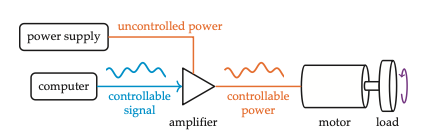
\includegraphics[width=.9\linewidth]{figures/motor_control.png}
	\caption{Typical motor-driving configuration using an signal to generate controllable power. \cite{Picone2024}.}
	\label{fig:motor-driving}
\end{figure}

The objectives of this lab are:
\begin{itemize}
	\item To implement a finite state machine control algorithm.
	\item To understand pulse-modulation driving of a DC motor.
	\item To use instruction timing to produce a calibrated delay
	\item To become familiar with qyadrature encoders
\end{itemize}

\section{Materials and Methods}

\subsection{Materials}
The materials used in this experiment were:
\begin{itemize}
	\item Windows 10 computer with myRIO support for C and Eclipse IDE.
	\item NI myRIO-1900
	\item Rigol DHO914S Digital Oscilloscope with $25 Mhz$ function generator
	\item Cables:
		\subitem BNC with alligator clips
		\subitem jumper cables
\end{itemize}

\subsection{Schematic of the equipment setup}

The schematic of the setup is shown in \autoref{fig:Schematic_DIO}. It shows the pins that are connected to the 
amplifier, buttons on the circuit board (stop and print), and the encoder.

\begin{figure}[htb]
	\centering
	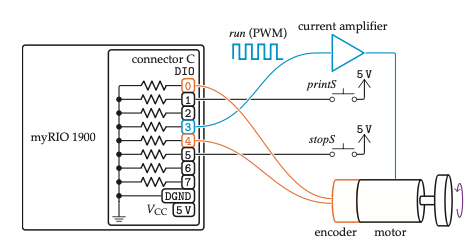
\includegraphics[width=.9\linewidth]{figures/Schematic_DIO_Output.png}
	\caption{Schematic of connection between the myRIO and the motor control circuit. \cite{Picone2024}.}
	\label{fig:Schematic_DIO}
\end{figure}

\subsection{Pulse-Width Modulation (PWM)}
A motor spins when current flows through its coils, thereby creating a magnetic field that produces
torque and therefore rotates the shaft.

More current results in more torque. An efficient way of control motor speed is by applying full voltage
but only part of the time. The N and M values in this lab represents the pulse width and period, respectively.

Example: N = 5, M=3

HIGH HIGH HIGH LOW LOW.

The motor spins smoothly and does not jerk ON and OFF because of motor physics. Motor
windings resist rapid current changes due to coil inductance so it does not stop instantly when power
goes off. Therefore, the motor experiences smooth continuous torque.

The motor behaves as if it is getting
\[
V_{\mathrm{avg}} = \left(\frac{N}{M}\right) V_{\max}
\]

Example: For a 5V system, N=5, M=3:
\[
V_{\mathrm{avg}} = \left(\frac{3}{5}\right) 5V = 0.6 \times 5V = 3.00V
\]
\subsection{Finite State Machine Implementation}

The Finite State Machine (FSM) implements the state transition logic depicted in
\autoref{fig:FSM}.

\begin{figure}[htb]
	\centering
	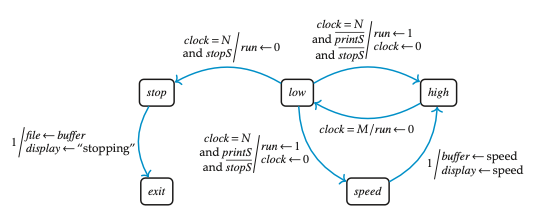
\includegraphics[width=.9\linewidth]{figures/State_Transition_Diagram.png}
	\caption{State Transition Diagram for the Finite State Machine. \cite{Picone2024}.}
	\label{fig:FSM}
\end{figure}

\section{Laboratory Exploration and Evaluation}

The complete source code for the lab is available on GitHub at \url{https://github.com/juliansoh/ME477/blob/main/workspace/Julian_lab4/main.c}.

\subsection{Problem L4.1}
Determine the exact number of clock cycles for the wait()
function of listing 4.2 to execute, accounting for all instructions (use table 4.6). From
that, calculate the delay interval in milliseconds. A spreadsheet is convenient for
making this calculation.

The mapping of the wait() function to assembly code is shown in \autoref{fig:Function-Assembly-mapping}.
The loop in the wait() function is highlighted in the dotted box and is the part of the code that executes 417000 times.

The setup overhead of the wait() function only runs once, as does the loop cleanup after i == 0.

\begin{figure}[htb]
	\centering
	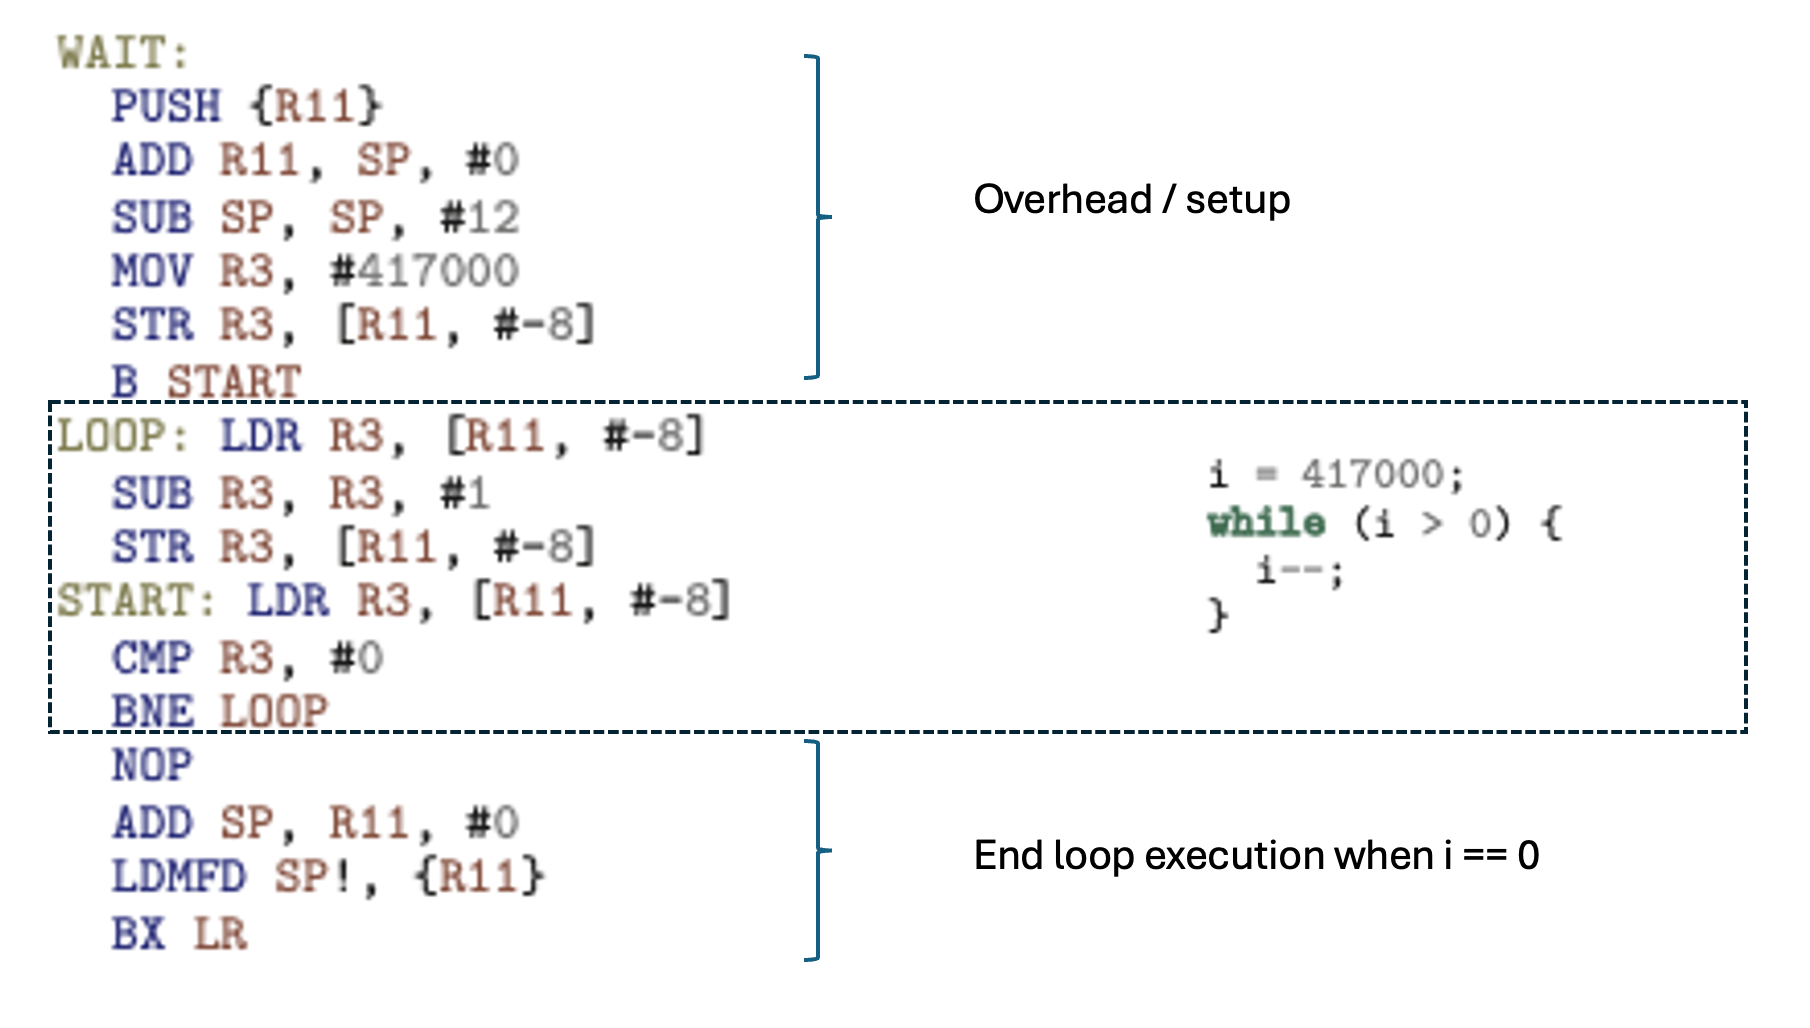
\includegraphics[width=.9\linewidth]{figures/Function-Assembly-mapping.png}
	\caption{Mapping the wait() to assembly code.}
	\label{fig:Function-Assembly-mapping}
\end{figure}


\begin{table}[h!]
\centering
\begin{tabular}{|c|c|c|}
\hline
\textbf{Instruction Type} & \textbf{Mnemonic} & \textbf{Clock Cycles} \\
\hline
Load/store registers & LDR, STR & 2 \\
\hline
Branch & BNE, B, BX & 0 \\
\hline
Stack & PUSH, LDMFD & 2 \\
\hline
Arithmetic & ADD, SUB, CMP & 1 \\
\hline
Move & MOV & 1 \\
\hline
No operation & NOP & 1 \\
\hline
\end{tabular}
\caption{Opcode execution times (CPU cycles) for instructions used in \texttt{wait()}}
\end{table}

\textbf{Function overhead/setup}

\begin{align*}
\text{PUSH} &: 2 \\
\text{ADD}  &: 1 \\
\text{SUB}  &: 1 \\
\text{MOV}  &: 1 \\
\text{STR}  &: 2 \\
\text{B}    &: 0
\end{align*}

\[
\text{Total setup cycles} = 2 + 1 + 1 + 1 + 2 = 7
\]

\textbf{Loop interation}
Each iteration of the loop executes the following instructions:

\begin{align*}
\text{LDR} &: 2 \text{ cycles} \\
\text{SUB} &: 1 \text{ cycle} \\
\text{STR} &: 2 \text{ cycles} \\
\text{LDR} &: 2 \text{ cycles} \\
\text{CMP} &: 1 \text{ cycle} \\
\text{BNE} &: 0 \text{ cycles}
\end{align*}

\noindent Total cycles per loop iteration:
\[
2 + 1 + 2 + 2 + 1 + 0 = 8 \text{ cycles}
\]

\noindent The loop executes $417000$ times, so total loop cycles:
\[
417000 \times 8 = 3,336,000 \text{ cycles}
\]

\textbf{Exit instructions:}
\begin{align*}
\text{NOP}   &: 1 \\
\text{ADD}   &: 1 \\
\text{LDMFD} &: 2 \\
\text{BX}    &: 0
\end{align*}

\[
\text{Total exit cycles} = 1 + 1 + 2 = 4
\]

Therefore, the total clock cycles for wait() is:
\[
\text{Total cycles} = 3,336,000 + 7 + 4 = 3,336,011 \text{ cycles}
\]

\textbf{Time Calculation}
The processor clock frequency is:
\[
f = 667\ \text{MHz}
\]

Clock period:
\[
T = \frac{1}{667 \times 10^6}
\]

Total execution time:
\[
t = \frac{3,336,011}{667 \times 10^6}
\]

\[
t \approx 0.00500\ \text{seconds} = 5.00\ \text{ms}
\]

\subsection{Problem L4.2}
Examine the circuit board attached to connector C of the myRIO.
The normally open push-button switches, when closed, connect DIO channels 1
and 5 to Vcc = 5 V when pressed, as shown in figure 4.19. Note: These channels have
pull-down resistors. Use the oscilloscope to view the waveform produced by your
program. For example, use N= 5, M= 3.

\vspace{\baselineskip}
From the oscilloscope, we observed the PMW waveform as shown in \autoref{fig:PWM_waveform}.

\begin{figure}[htb]
	\centering
	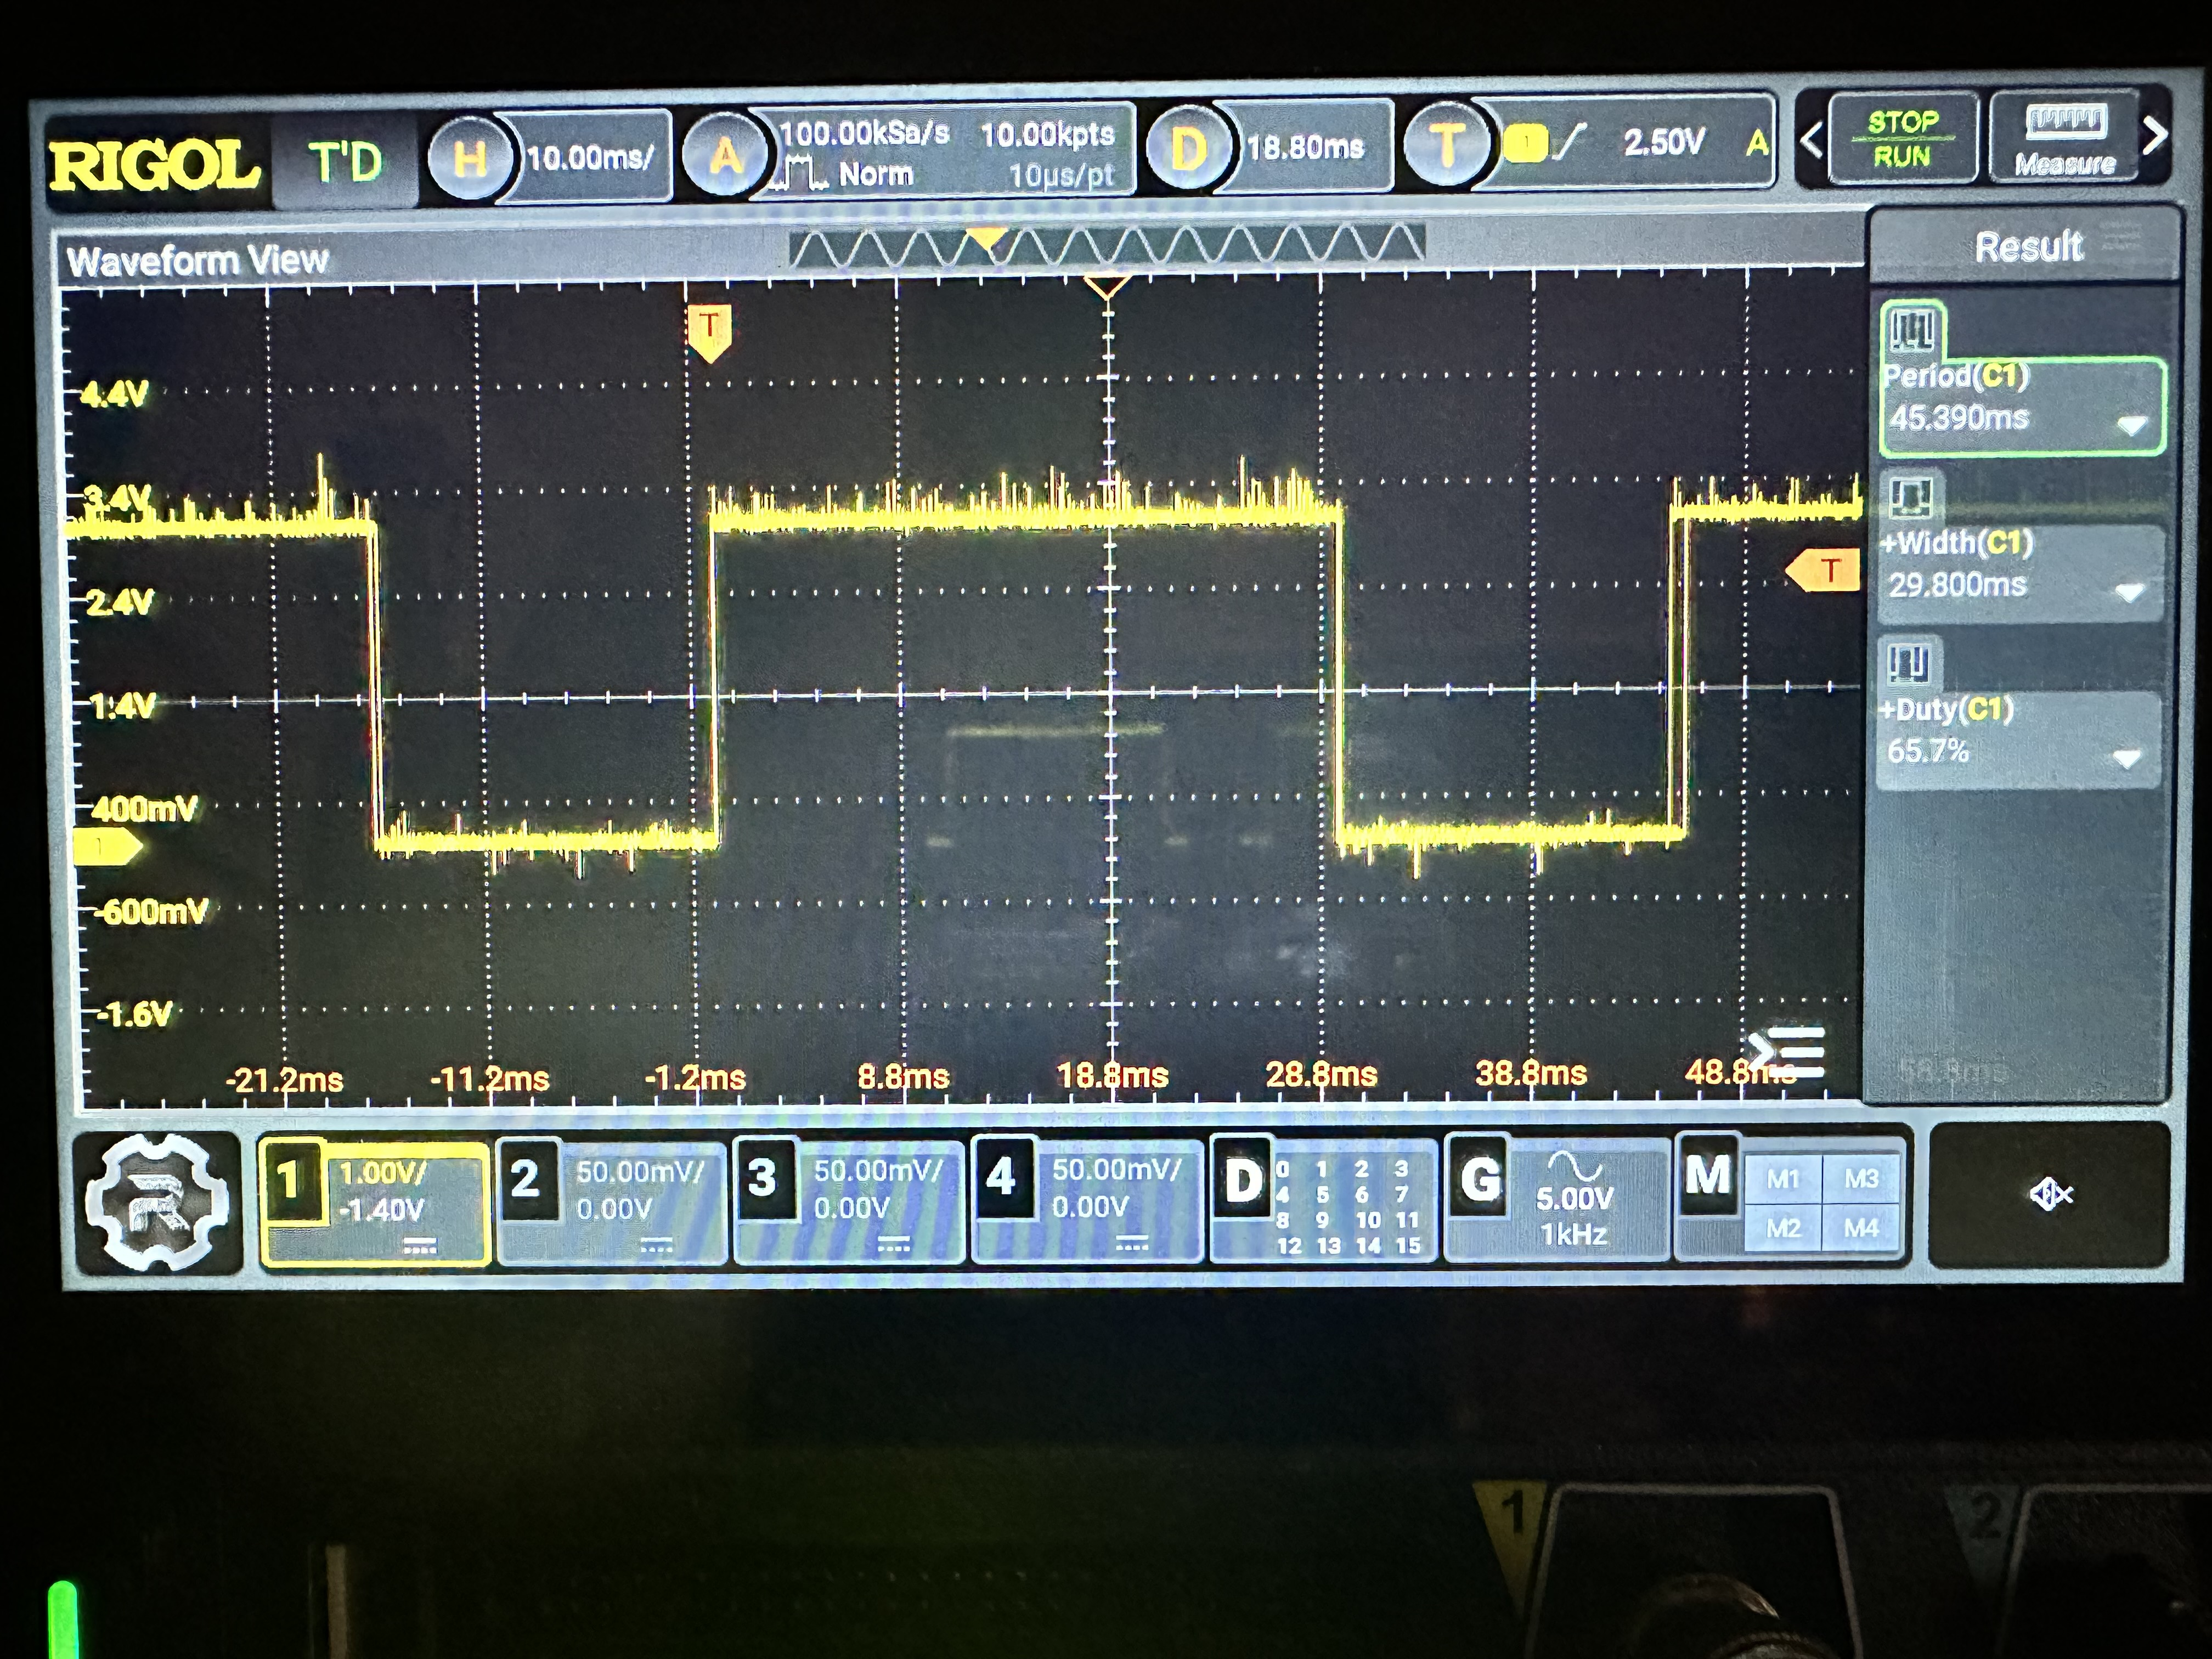
\includegraphics[width=.9\linewidth]{figures/PWM_waveform.jpeg}
	\caption{Image of the PWM waveform from the Oscilloscope.}
	\label{fig:PWM_waveform}
\end{figure}

\subsection{Problem L4.3}
Compare your program's printed output (on the LCD) to the
steady state motor speed as measured with an optical tachometer.

\subsection{Problem L4.4}
Use the oscilloscope to view the PWM waveform produced by
your program, and to measure the actual length of a BTI. Is it what you expect? If
not, why not?

\vspace{\baselineskip}
Refer to \autoref{fig:PWM_waveform} again and note the measurements taken on the waveform were:
\begin{itemize}
	\item Period: $46\ \mathrm{ms}$ ($N$)
	\item Width (high): $30\ \mathrm{ms}$ ($M$)
	\item Duty cycle: $65\%$
	\item $M/N = 30/46 = 0.65$
\end{itemize}

We entered N=5 and M=3, so the expected duty cycle is 3/5 = 0.6 or 60\%. 
The actual duty cycle is 65\%, which is slightly higher than expected. This could be due to timing inaccuracies in the program or the oscilloscope measurements.


\subsection{Problem L4.5}
Repeat lab problem L4.4 while printing the speed (pressing
the switch). What does the oscilloscope show has happened to the length of the
BTI? What's going on!?

\vspace{\baselineskip}

When the print button is pressed, the oscilloscope shows that the length of the BTI (Base Time Interval) has changed. 
The new measured values were:
\begin{itemize}
	\item Period: $56\ \mathrm{ms}$ ($N$)
	\item Width (high): $46\ \mathrm{ms}$ ($M$)
	\item Duty cycle: $81\%$
	\item $M/N = 46/56 = 0.82$
\end{itemize}

\subsection{Problem L4.6}
Describe how you made the measurements of lab problems L4.4
and L4.5 and discuss any limitations in the accuracy of the timing of the output. In
lab exercise 6, we will find ways of overcoming this limitation.

\vspace{\baselineskip}
Refer to \autoref{fig:PWM_waveform} that shows the screen of the oscilloscope. The measurements
taken are shown to the right of the waveform: Period, +Width, and +Duty.

These measurements were taken by using the oscilloscope's measurement tools and selecting
these parameters from the oscilloscope's menu.

The limitations of using these tools is that the measurements are taken in real time
and may be subject to noise and other sources of error. We could just take the average
of the measurements to improve accuracy. Nevertheless, this approach is more accurate than 
manual measurements or visual inspection.

\subsection{Problem L4.7}
After you have your code running as described above, try this:
Record the velocity step response of the DC motor, save it to a file, and plot it in
MATLAB. Here's how:

\subsection{Problem L4.8}
You may have noticed that when M = 1, the FSM does not
function as desired. Address the following issues:
\begin{enumerate}
	\item What is wrong?
	\item How would modifying the state transition diagram correct this problem?
	\item How would you modify the state transition table?
	\item Modify your program to correct the $M = 1$ case. Test the result.
\end{enumerate}

\subsection{Problem L4.9}
A programmer has written following code in an attempt to
initialize the encoder.
\begin{lstlisting}[language=C]
MyRio_Encoder *encC0;
EncoderC_initialize(myrio_session, encC0);
\end{lstlisting}
It's incorrect. What issues could this code cause, and why?

\vspace{\baselineskip}
The declaration initializes a pointer to the \texttt{MyRio\_Encoder} structure but does not allocate
memory for the structure itself. Therefore, when the code attempts to read or write
to this memory location, it will access invalid or nonexistent memory.

Instead, the \texttt{MyRio\_Encoder} structure should be declared. The address operator
can then be used to pass a pointer to the \texttt{MyRio\_Encoder} structure. See page 230
of~\cite{Picone2024}.

\section{Author Contributions}

There is only one author for this report and lab.



%%% References -------------------------

\bibliographystyle{plainnat}
\bibliography{report}

%%% Appendices -------------------------

\end{document}  